En esta sección mostramos y detallamos el diagrama entidad relación. Dado el tamaño del mismo se opto por separarlo y
centrar cada parte en una o dos entidades si sus interrelaciones.

\begin{figure}[H]
  \centering
    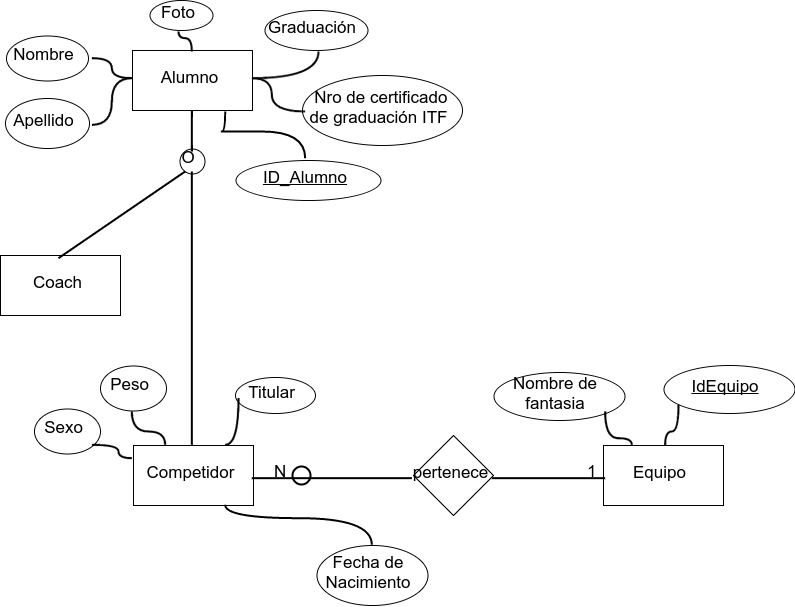
\includegraphics[scale=0.5]{imagenes/AlumnoCompetidor.png}
  \caption{Diagrama centrado en Alumno y Competidor}
\end{figure}

Los alumnos pueden adoptar el rol de un competidor o del coach. A su vez, un competidor puede, o no, formar parte de un equipo
. Se distinguen a los competidores pertenecientes a un equipo por su atributo titular, este indica si se trata de un titular
del equipo o un suplente. En el caso de que no pertenezca a ningún equipo, el atributo titular queda vacío.

\begin{figure}[H]
  \centering
    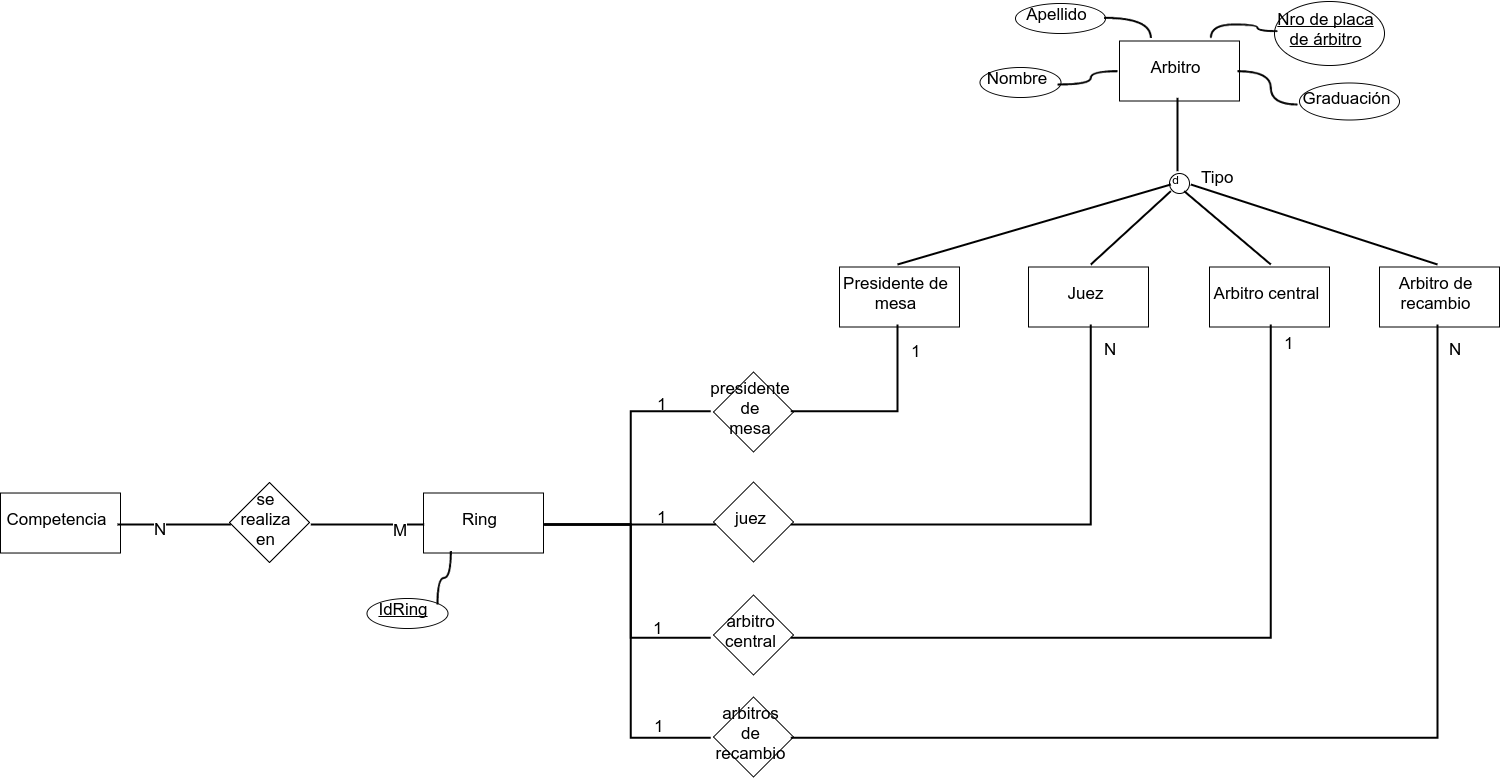
\includegraphics[scale=0.3]{imagenes/ArbitroRing.png}
  \caption{Diagrama centrado en Árbitro y Ring}
\end{figure}

Un árbitro puede ser un presidente de mesa, juez, árbitro central o árbitro de recambio. Cada ring posee un presidente de mesa
y un árbitro central, dependiendo de la competencia varía la cantidad de árbitros correspondientes a los otros tipos.
Un Ring también está asociado a una o más competencias, a su vez para realizar una competencia se podría necesitar de  varios
rings(al menos uno).

\begin{figure}[H]
  \centering
    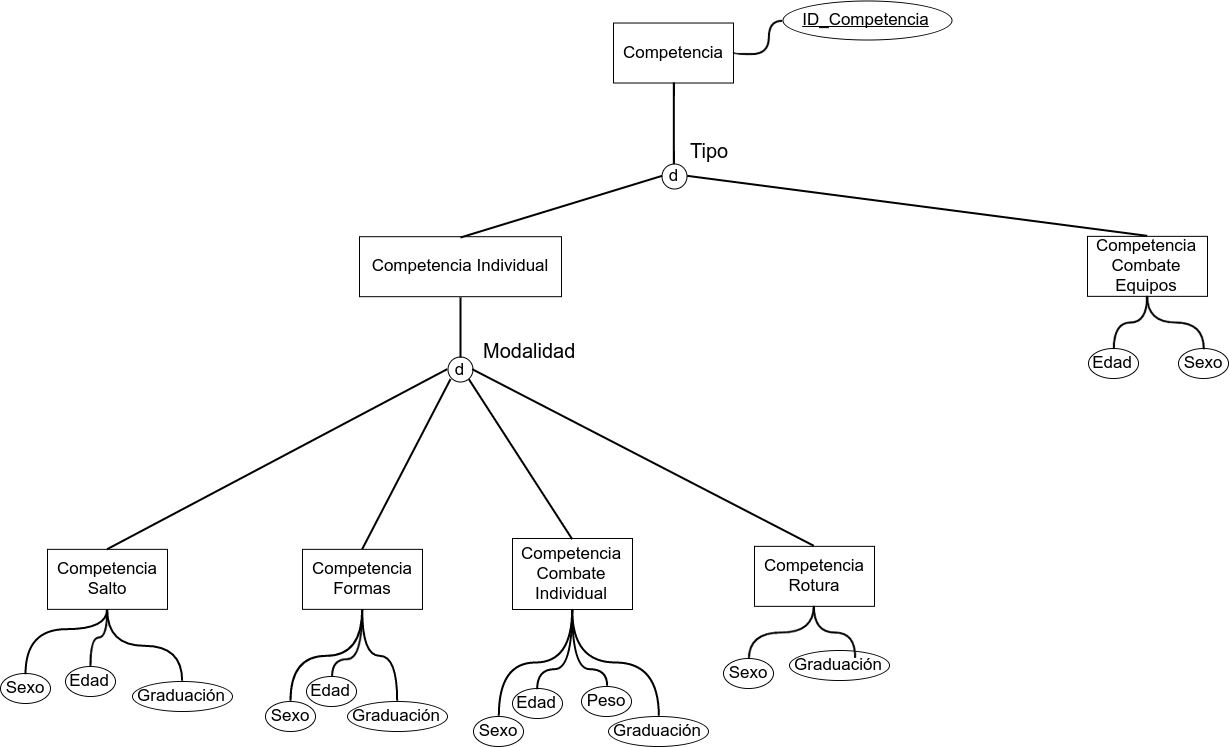
\includegraphics[scale=0.3]{imagenes/Competencia.png}
  \caption{Diagrama centrado en Competencia}
\end{figure}

Las competencias se dividen entre las que son individuales y en las cuales participan equipos. De esta última solo se tiene
 como modalidad a las competencias de combate por equipos, en cambio las competencias individuales poseen 4
 modalidades diferentes. Estas son Salto, Formas, Combate individual, Rotura. Cada una con sus parámetros de participación
 (sexo, edad, etc).

\begin{figure}[H]
  \centering
    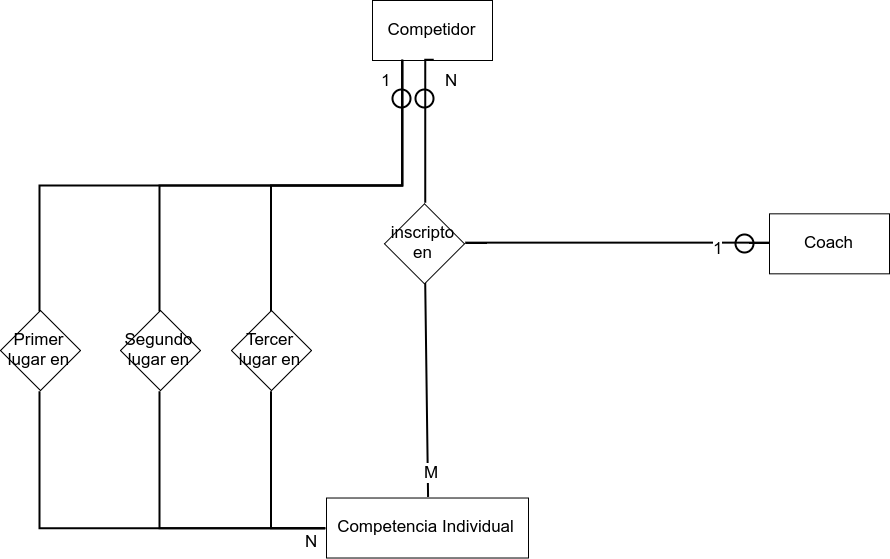
\includegraphics[scale=0.5]{imagenes/CompetidorCompetencia.png}
  \caption{Diagrama centrado en Competidor y Competencia}
\end{figure}

Los competidores se pueden inscribir en una o varias competencias individuales, esto lo hacen supervisado por un coach. A su
vez, el coach puede tener varios de sus competidores inscriptos a una misma competencia. Cada competencia registra a los
competidores que quedaron en los primeros tres lugares.

\begin{figure}[H]
  \centering
    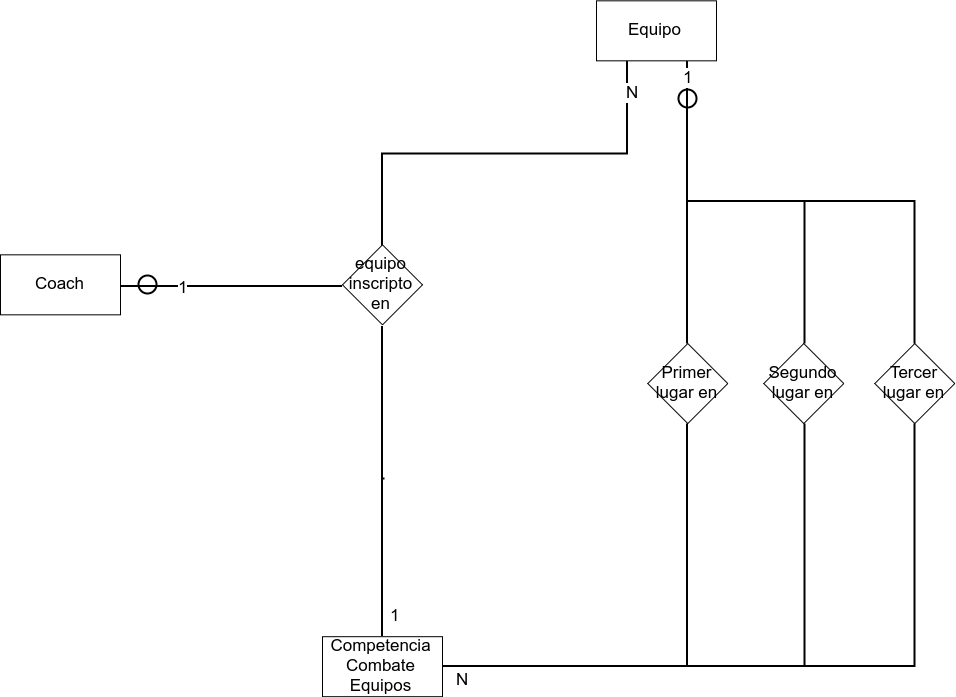
\includegraphics[scale=0.5]{imagenes/EquipoCompetencia.png}
  \caption{Diagrama centrado en Equipo y Competencia}
\end{figure}

Similar que el anterior, pero con las competencias por equipos. La principal diferencia es que en la inscripción, debido a
la cantidad de miembros que deben componer un equipos y la cantidad de competidores que puede supervisar un coach, solamente puede quedar inscripto un equipo por cada
coach en una determinada categoría.

\begin{figure}[H]
  \centering
    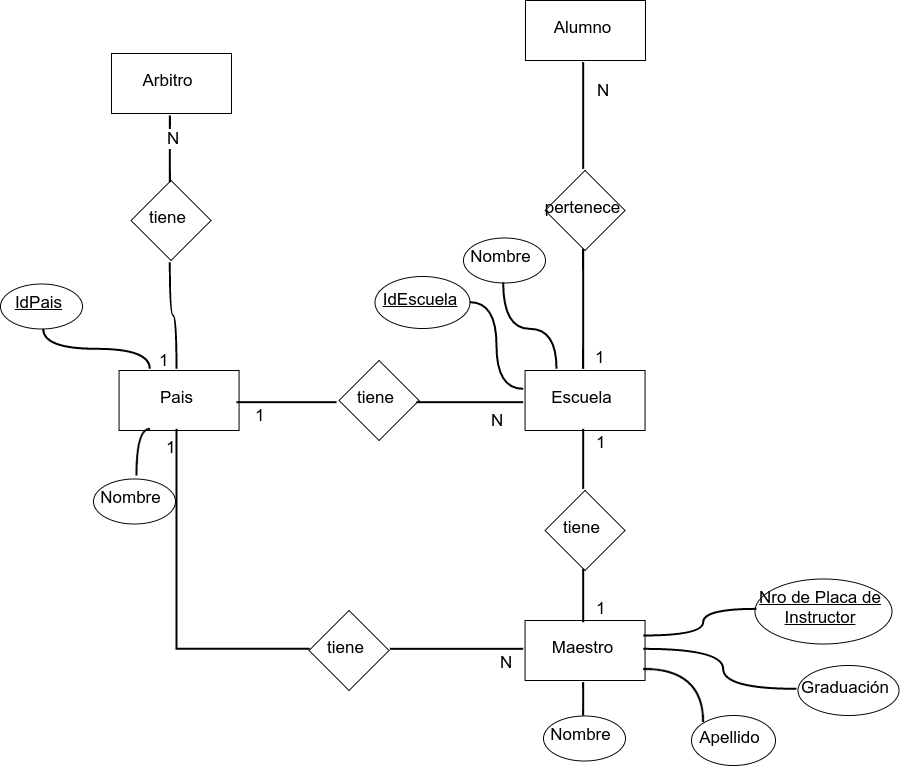
\includegraphics[scale=0.5]{imagenes/EscuelaPais.png}
  \caption{Diagrama centrado en Escuela y País}
\end{figure}

Por último tenemos que tanto Maestros, Árbitros y Escuelas proceden de determinados países. Además cada
escuela posee alumnos y a un maestro que se encarga de la inscripción de los mismos en las competencias.
